\chapter{Heart rate sensor}\label{ch:heartRate}
%**********************************************

%**********************************************
\section{Introduction} \label{sec:heartIntro}
%**********************************************


Introduce the reader to what you want to present in this chapter. 
Include any references to literature you feel is needed. 
In this section, you put a very short summary of infrormation you gatherered from literature (papers, web sites, datasheets) that you used to do the design. Be sure to include the references, which you can add in the \texttt{References.bib} file. 
Rather than just copy\&pasting \footnote{I have a little bee in my bonnet about people who say ``cut\&paste'' - if it were cut, it would not be there anymore!} from the datasheet, give your own circuit diagrams. Remember, it is important that someone who reads your report must be able to reproduce your results. 

Some examples of how to cite (all in \texttt{References.bib}): 
It was stated by \cite{Booysen:2013} that ... . Subsequently, he changed his mind and said in  \cite{Gerber:2019} that ... .
While \cite{WebsiteOpAmp} claims it to be ... .


%**********************************************
\section{Design} \label{sec:heartDesign}
%**********************************************

In this section, you need to capture your design, which should include the following: 
\begin{itemize}
  \item Design rationale, i.e. what your thinking was behind the design. For example, explain that you had to first analyse the heart beat signals before you could design the filtering. 
  \item References to literature/sources as appropriate \cite{WebsiteOpAmp}.  
  \item You can assume the reader has an E\&E degree, and will not need detail explanations of trivial information (e.g. what a resistor is, or what Ohm's law is).  
  \item Design calculations, for example to determine resistor values and capacitor values, or to check for allowed voltage and current ranges and levels. These calculations should also give expected outputs, which hopefully matches the simulated values. Importantly, they are based on maths, and not on simulation - there is a difference. 
  \item Analysis of given or expected input conditions. 
  \item Expected values and ranges based on your design. 
  \item Explain your choice of supply buy referring to the advantages and disadvantages of each. 
  \item Circuit diagram like the one in Figure \ref{fig:circuit_diagram}. I used ``print to PDF'' from LTSpice,  but feel free to use a cropped screengrab if you are PDF-challenged and do not have a PDF printer (there are some free PDF creators online). Also have a look at the demo video on SUNLearn. 
\end{itemize}

For your benefit, here is how to write values with units: \SI{150}{\milli\Omega} or \SI{199}{myUnits}, and this is how we write ranges: \numrange{2}{5} \si{\kilo\volt}.

Here is an inline equation $ \frac{55}{45+3}$. Here is a numbered equation in Eq. \ref{eq:myNumberedEquation}.
\begin{equation}
   a = \frac{55}{45+3}
   \label{eq:myNumberedEquation}. 
\end{equation}. 

\begin{figure}
 \footnotesize
   \centering
   \begin{subfigure}[]{0.45\textwidth}
        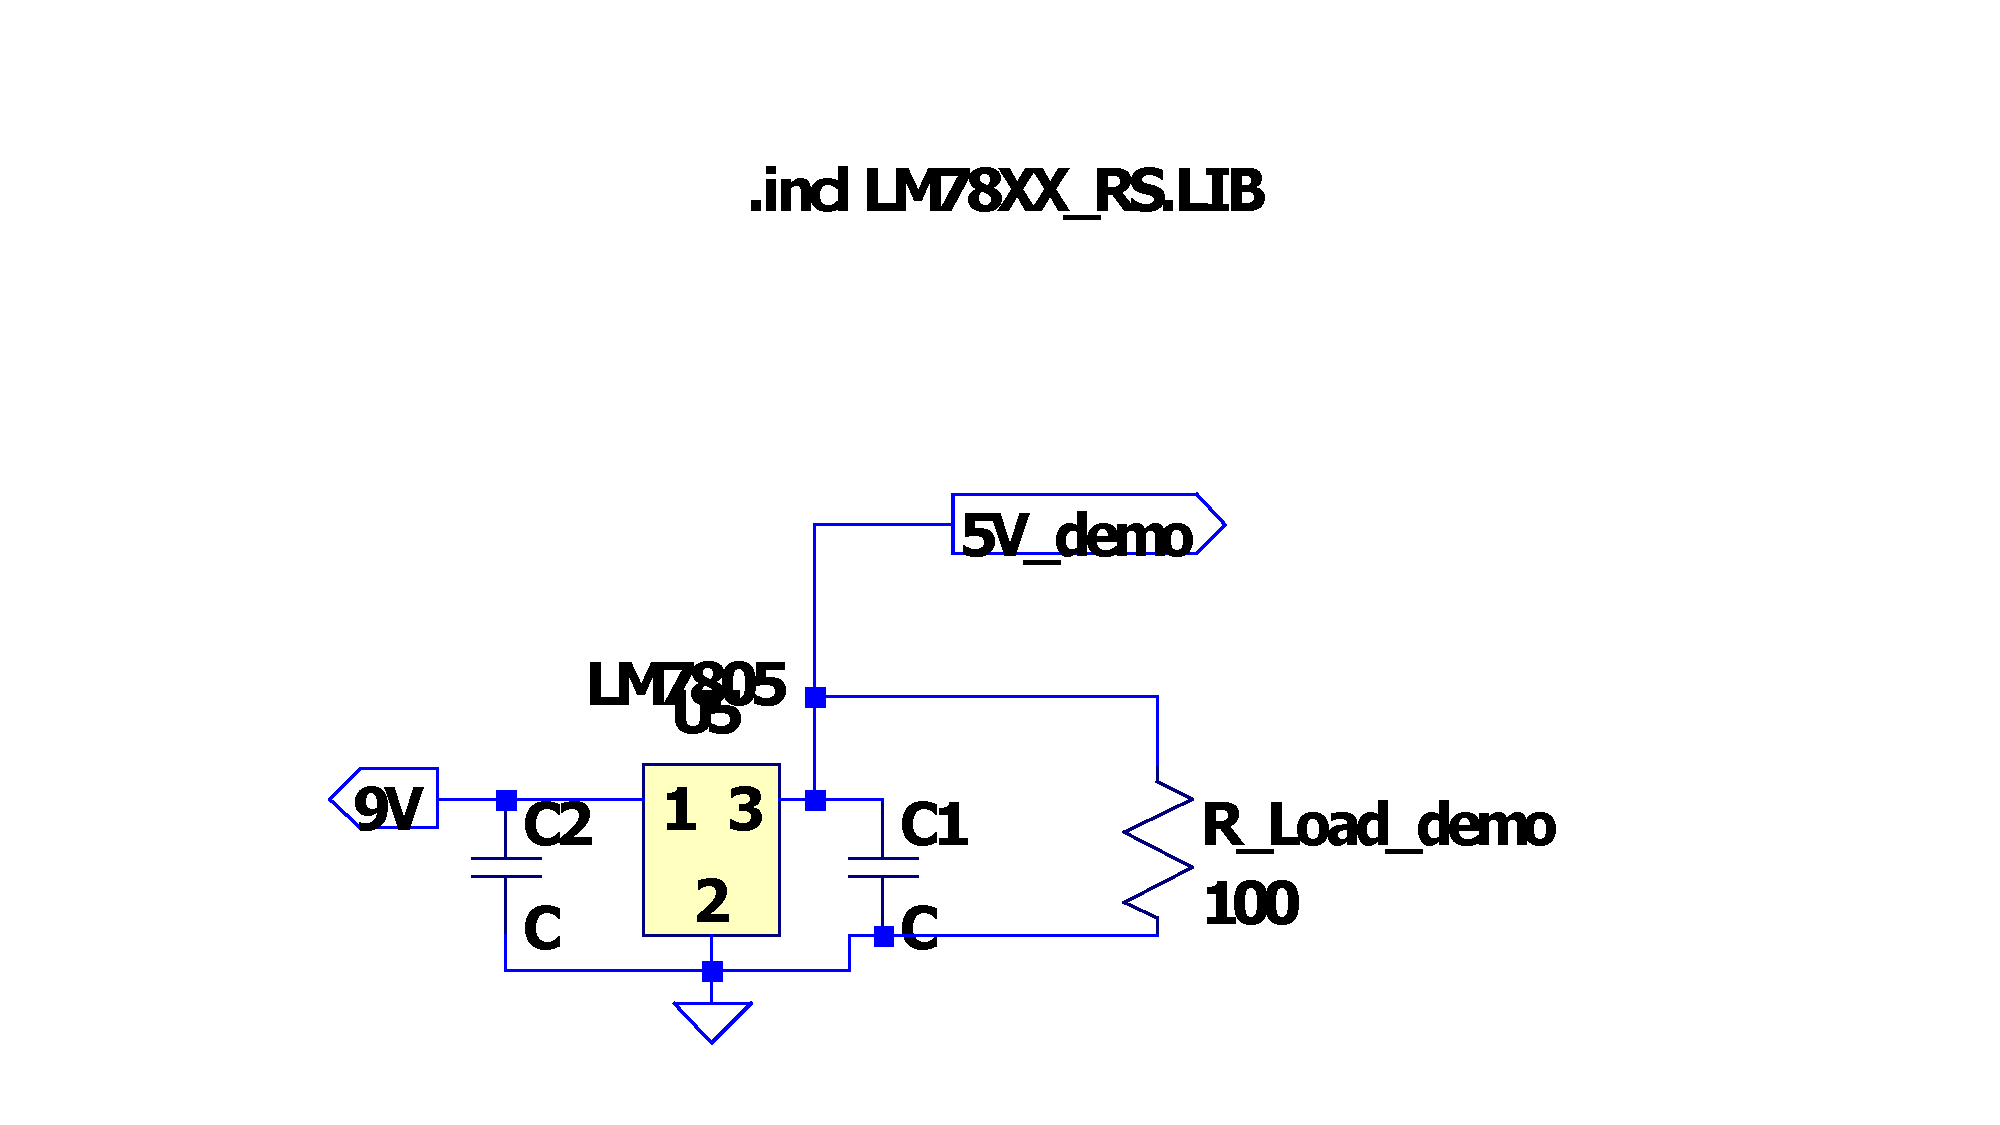
\includegraphics[width=\linewidth]{./Figures/E344_Ass1VoltRegulator_cct}
	  \caption{Linear voltage regulator.} \label{subfig:linear_circuit_diagram}	
   \end{subfigure}
   \begin{subfigure}[]{0.45\textwidth}
  	 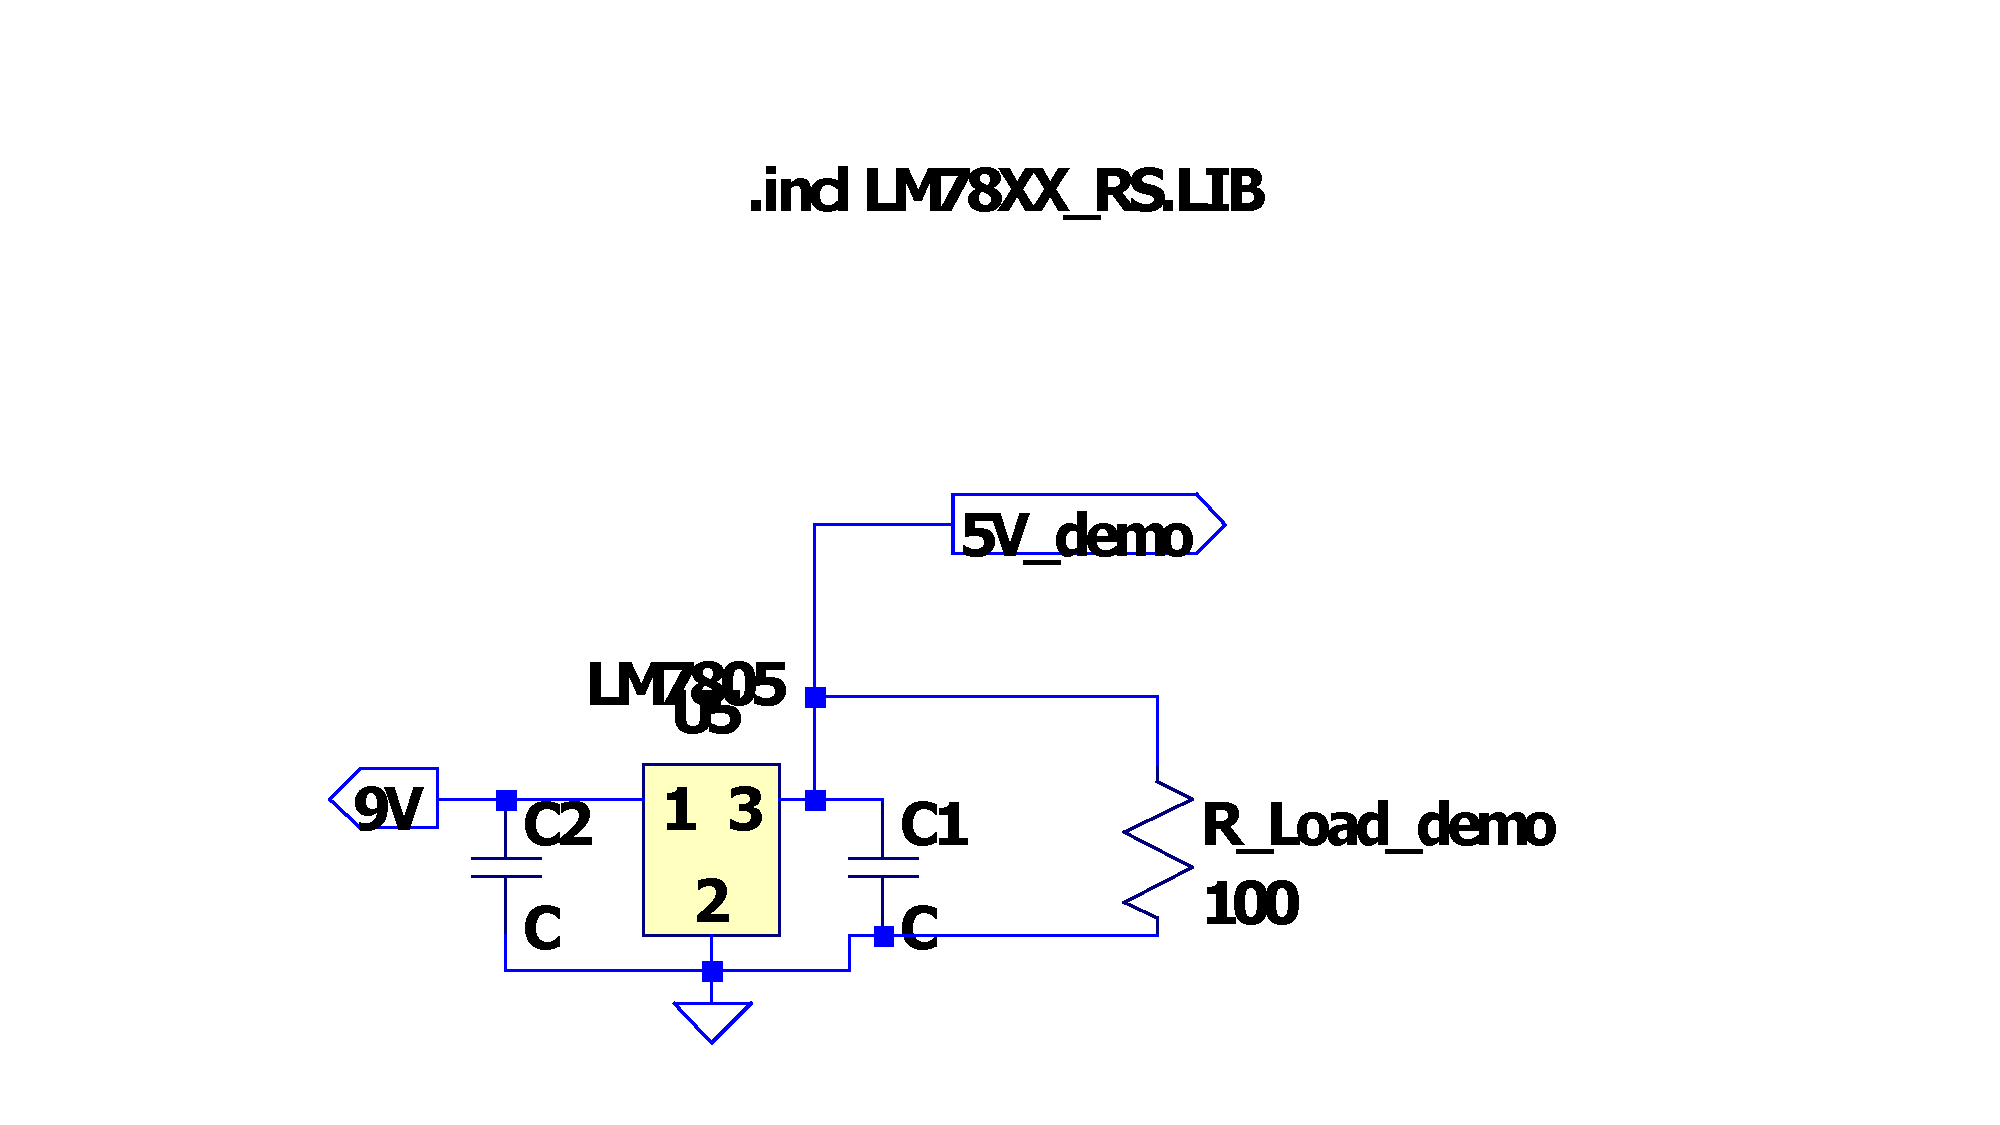
\includegraphics[width=\linewidth]{./Figures/E344_Ass1VoltRegulator_cct}
	  \caption{Switchmode voltage regulator.} \label{subfig:switchmode_circuit_diagram}	
   \end{subfigure}
   \begin{subfigure}[]{0.95\textwidth}
  	 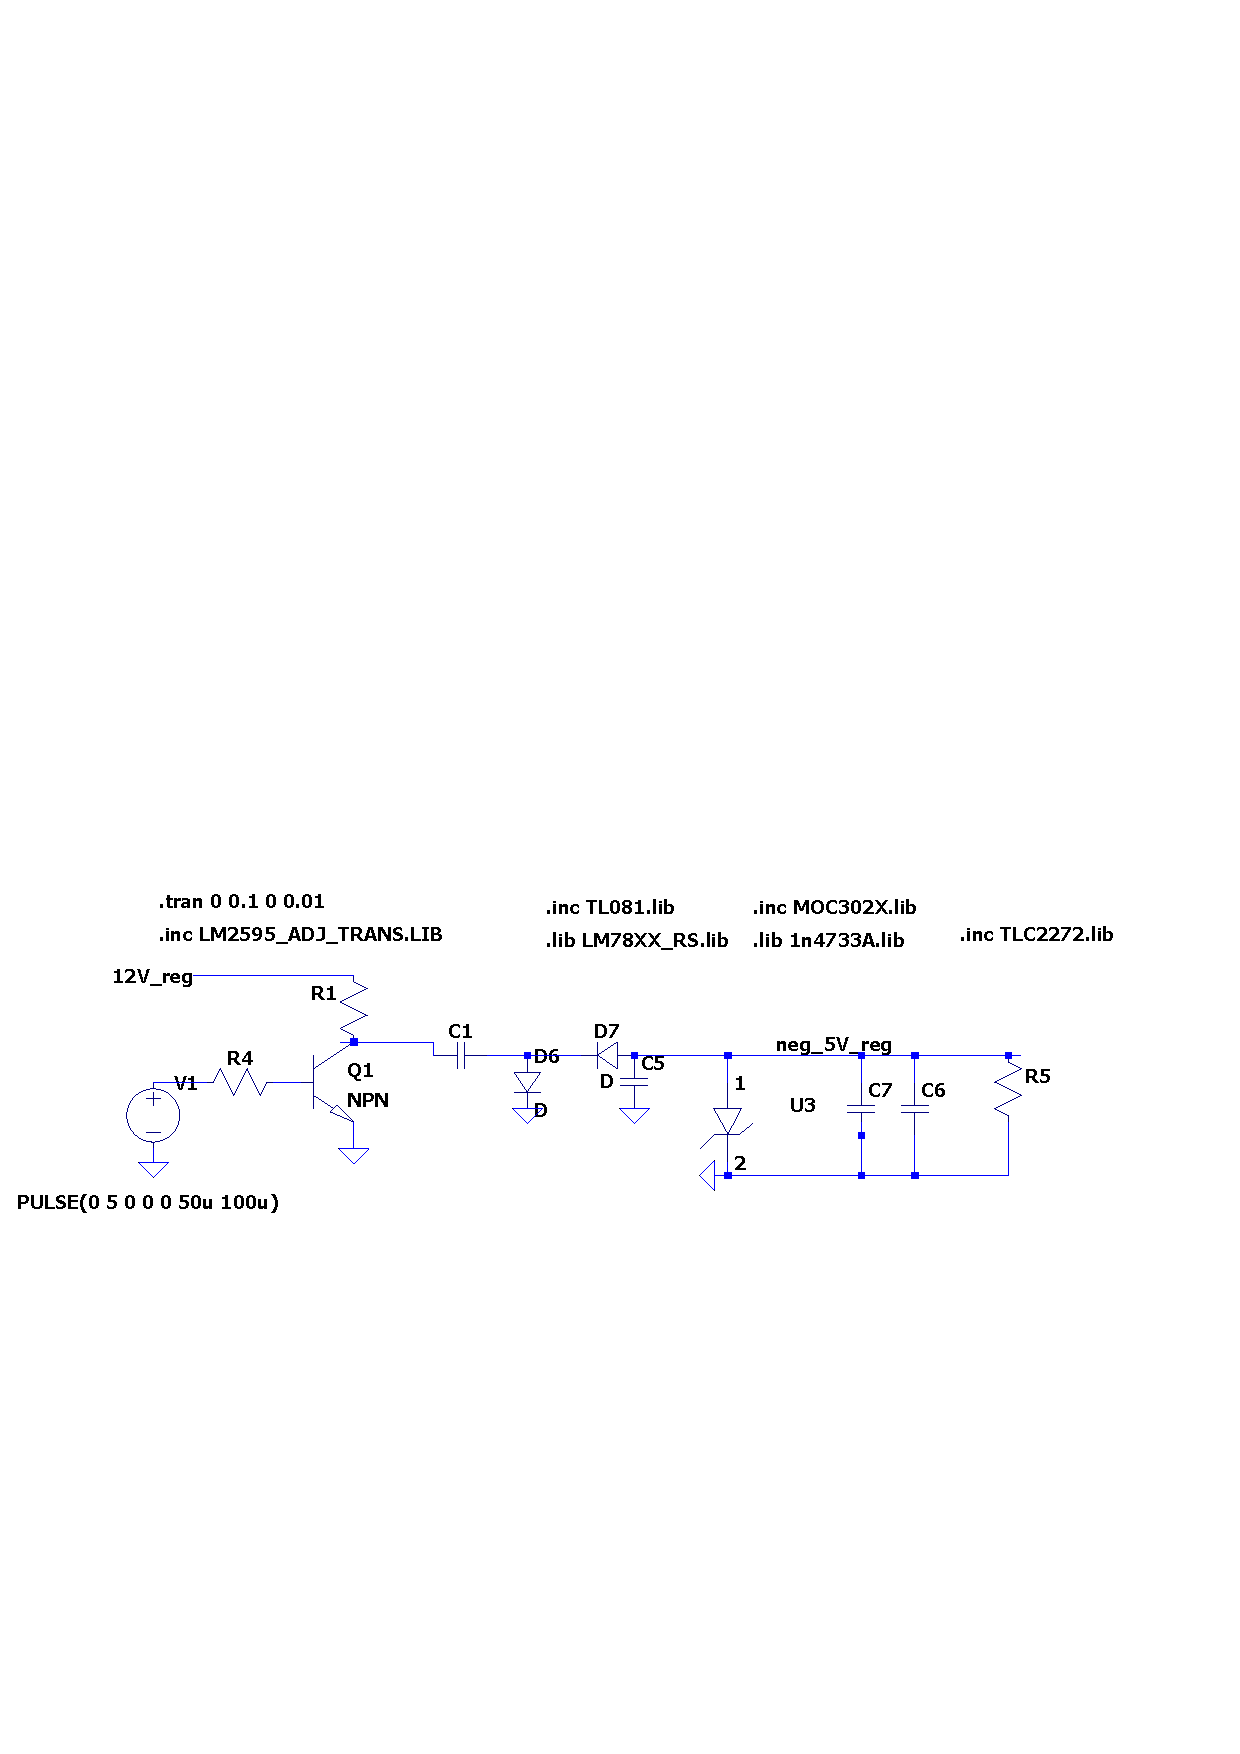
\includegraphics[width=\linewidth]{./Figures/CctDia}
	  \caption{Chargepump voltage regulator.} \label{subfig:chargepump_circuit_diagram}	
   \end{subfigure}
   
   \caption {Circuit diagrams of the two voltage regulators, and another irrelevant one}.

      \label{fig:circuit_diagram}
 \end{figure}
%**********************************************
\section{Results} \label{sec:heartResults}
%**********************************************


\begin{figure}
 \footnotesize
 \centering
    \begin{subfigure}[]{0.55\textwidth}
              \centering
  		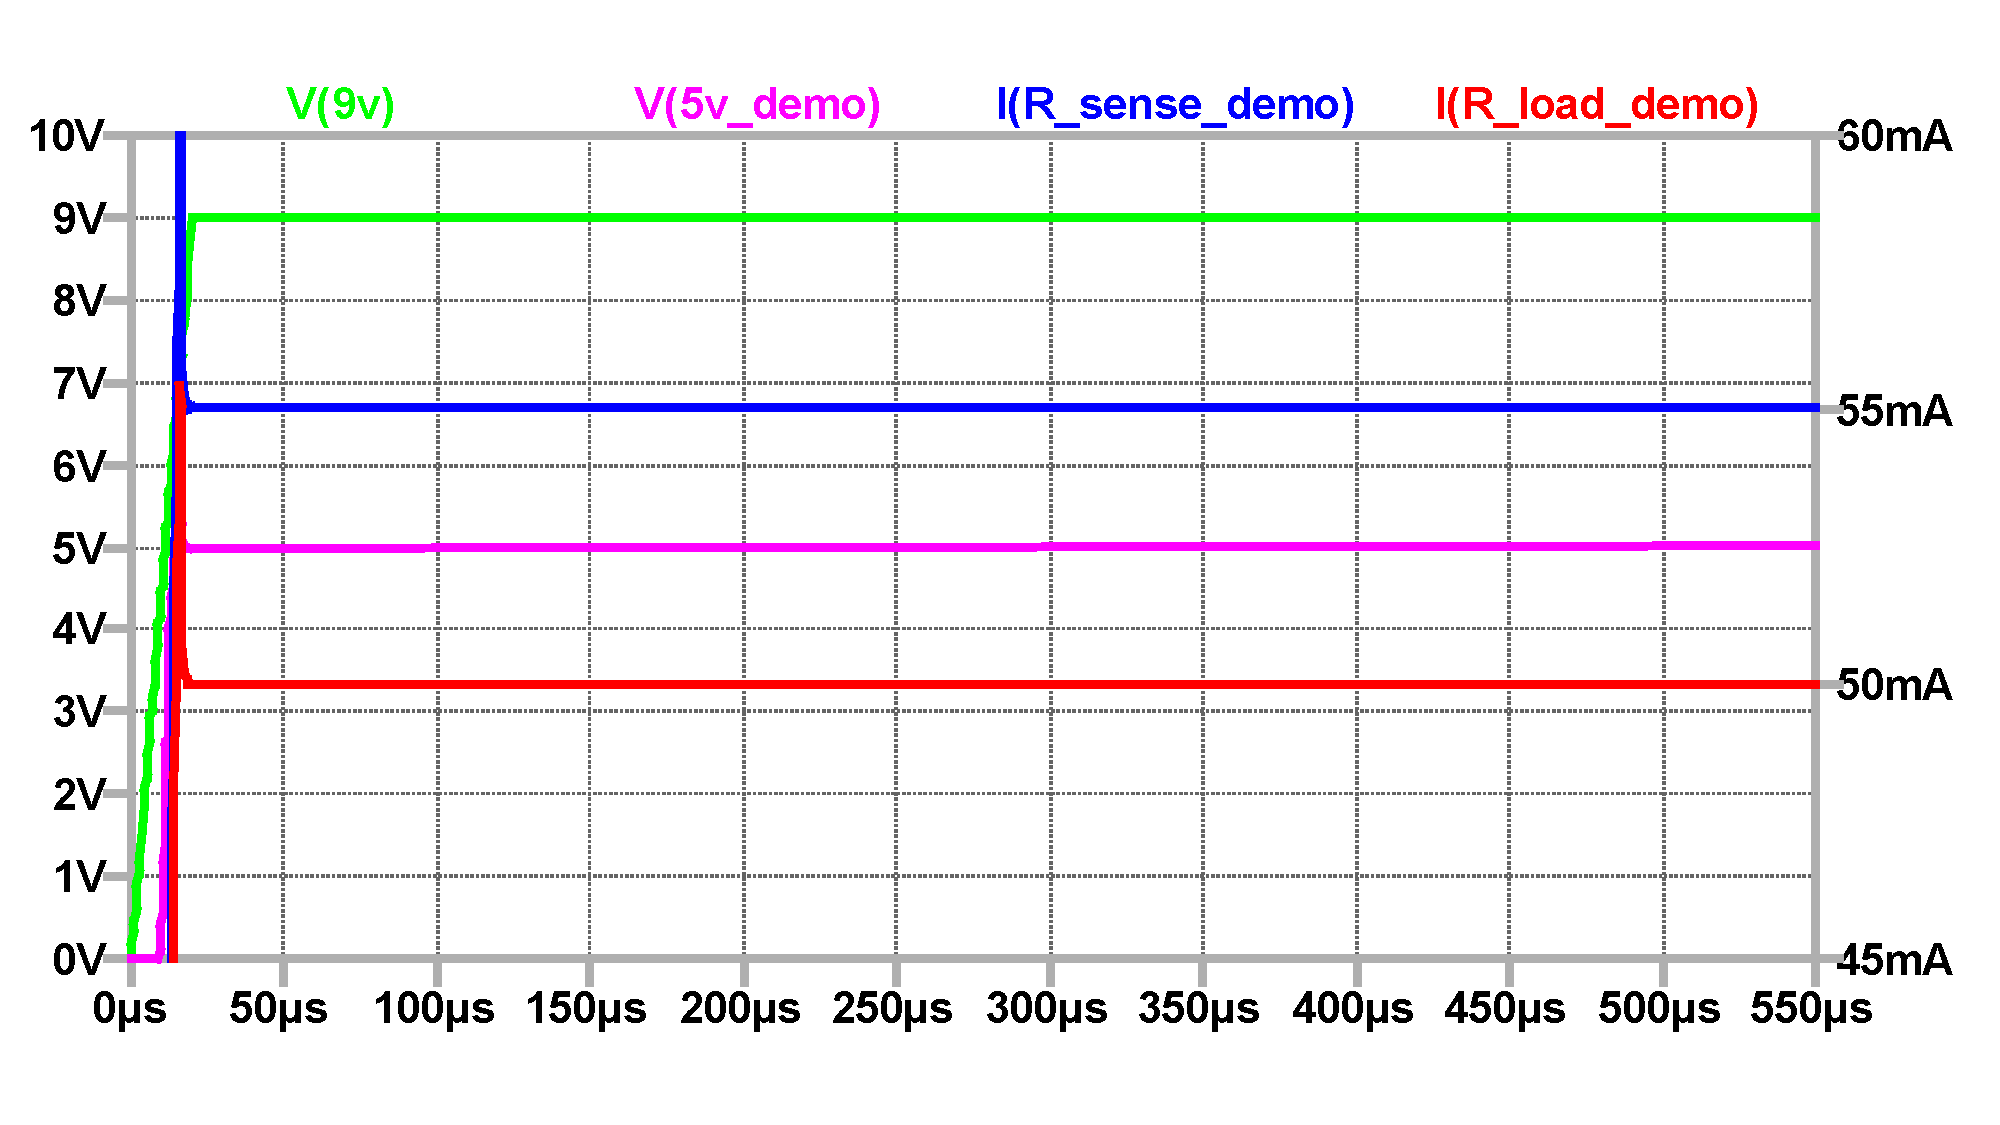
\includegraphics[width=1\linewidth]{./Figures/E344_VoltRegulator.pdf}
		    \caption{} \label{subfig:pwr_simu_rect}
     \end{subfigure}
     \begin{subfigure}[]{0.4\textwidth}
             \centering
  		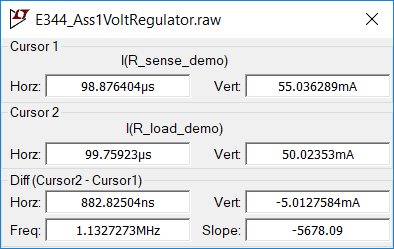
\includegraphics[width=1.0\linewidth]{./Figures/Screengrab2}
		   \caption{ } \label{subfig:pwr_meas_rect}
     \end{subfigure}
    \begin{subfigure}[]{0.55\textwidth}
              \centering
  		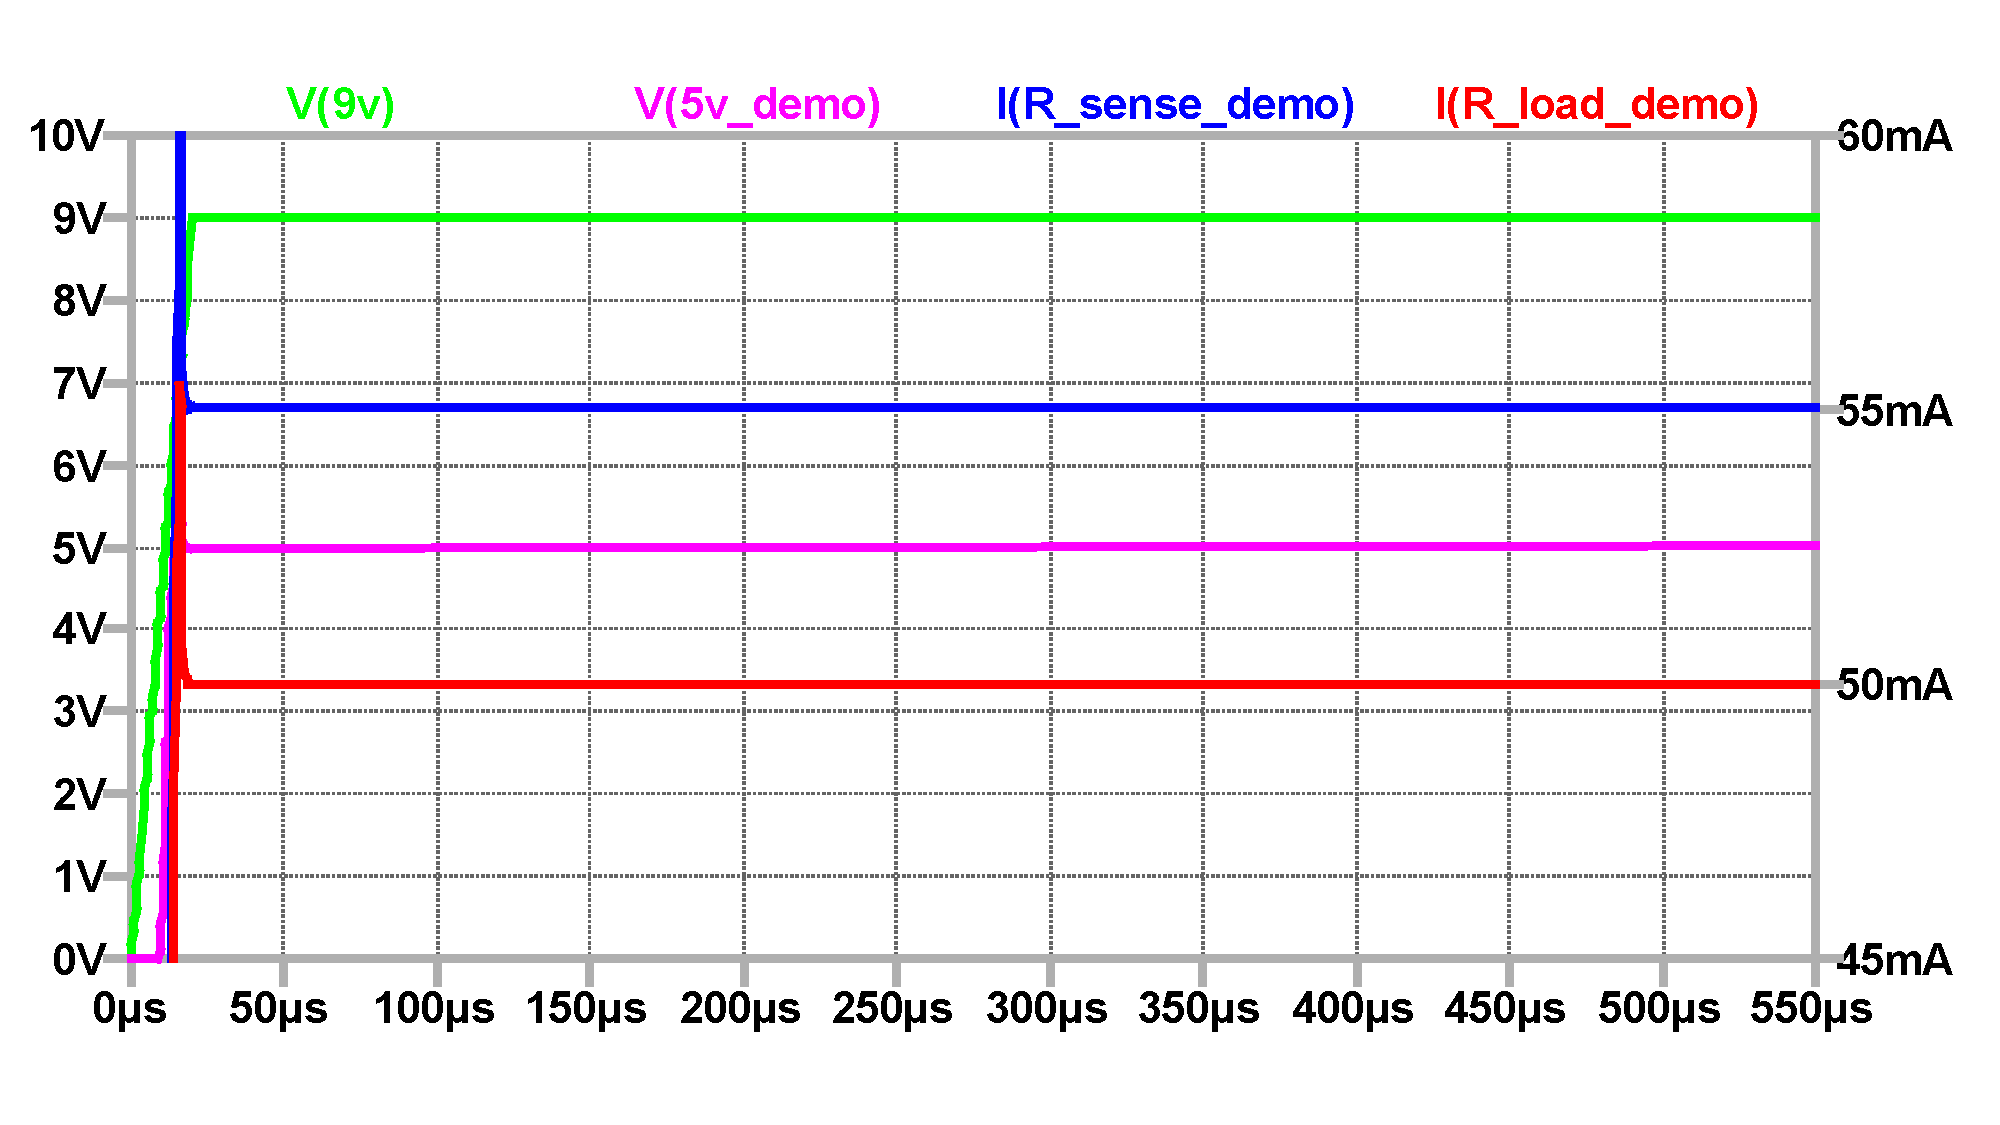
\includegraphics[width=1\linewidth]{./Figures/E344_VoltRegulator.pdf}
		    \caption{} \label{subfig:pwr_simu_rect}
     \end{subfigure}
    \begin{subfigure}[]{0.4\textwidth}
              \centering
  		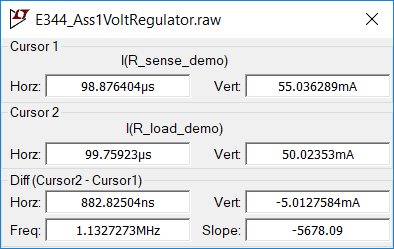
\includegraphics[width=1\linewidth]{./Figures/Screengrab2}
		    \caption{} \label{subfig:pwr_simu_rect}
     \end{subfigure}
   \caption[\textcolor{red}{I am the short caption that appears in the List of Figures list}]{Voltage regulation, comparing the linear and switchmode regulators... (a)  Blah blah. (b)  Blah blah.  (c)  Blah blah. (d) Blah blah.   As far as possible, please put input(s) and output(s) on the same plot rather than on separate plots. Based on the datasheet of XXXX in \cite{WebsiteOpAmp}}
    \label{fig:simulation_results_box}
 \end{figure}

In this section, you want to demonstrate, by means of referring to simulation results, using the designed circuit, how your circuit behaves as you designed it in Section \ref{sec:heartDesign}. Present and report on your simulated results in Figure \ref{fig:simulation_results_box}. Be absolutely sure that the text and information in your report are readable. 

You can use screengrabs or photos of the oscilloscope, or download the CSVs and plot them as PDFs using Matlab, Excel or similar. 
You can also use tables, example of which are presented in Tables \ref{tab:table1} and \ref{tab:table2}.


\begin{table}
        \centering
        \footnotesize
        \caption{Example of a simple table.}
         \begin{tabular}{c@{\qquad}rrrr}
          \toprule
             & 2017 & 2018 & $\Delta_{Abs}$ & $\Delta_{DiD}$\\
          \midrule
          A & 9,868      & 10,399 & +5 & -11\\
          B & 10,191     & 10,590 & +4 & -12\\
          \bottomrule
        \end{tabular}
     \label{tab:table1}
\end{table}


\begin{table}
         \centering
        \footnotesize
        \caption{Example of another table.}

         \begin{tabular}{c@{\qquad}rrrr}
          \toprule
          \multirow{2}{*}{\raisebox{-\heavyrulewidth}{Schools }} & \multicolumn{2}{c}{Total energy used}& \multicolumn{2}{c}{Change}\\
          \cmidrule{2-5}
            & 2017 & 2018 & $\Delta_{Abs}$ & $\Delta_{DiD}$\\
            & [kWh] & [kWh] & [\%] & [\%] \\
          \midrule
          A & 9,868      & 10,399 & +5 & -11\\
          B & 10,191     & 10,590 & +4 & -12\\
          \bottomrule
        \end{tabular}
     \label{tab:table2}
\end{table}


%**********************************************
\section{Summary}\label{sec:temp_summary}
%**********************************************
State whether your design performs as expected and what the limitations are or things to keep in mind are. 


